\documentclass[conference]{IEEEtran}
\IEEEoverridecommandlockouts
% The preceding line is only needed to identify funding in the first footnote. If that is unneeded, please comment it out.
\usepackage{cite}
\usepackage{amsmath,amssymb,amsfonts}
\usepackage{algorithmic}
\usepackage{graphicx}
\usepackage{textcomp}
\def\BibTeX{{\rm B\kern-.05em{\sc i\kern-.025em b}\kern-.08em
    T\kern-.1667em\lower.7ex\hbox{E}\kern-.125emX}}
\begin{document}

\title{Propasal for Solving Mutliplayer Snake using Compitive Self-play Reinforcement Learning}

\author{\IEEEauthorblockN{Nitesh Kumar Rath}
\IEEEauthorblockA{\textit{University  of Florida}\\
nitish.rath@ufl.edu}
\and
\IEEEauthorblockN{Srajan Paliwal}
\IEEEauthorblockA{\textit{University of Florida}\\
srajanpaliwal@ufl.edu}
\and
\IEEEauthorblockN{Sourav Dutta}
\IEEEauthorblockA{\textit{University of Florida}\\
duttasourav@ufl.edu}
}

\maketitle

\begin{abstract}
This project aims at solving one of the open research problems published by OpenAI\cite{n3}. This project is focused on implementing a multi-player clone of a Snake game based on the online hit \textit{slither.io}. The project aims to explore various reinforcement learning methodologies to solve the problem. This makes use of Gym toolkit by openAI as a base for reinforcement learning. 
\end{abstract}

\begin{IEEEkeywords}
deep learning, reinforcement learning
\end{IEEEkeywords}

\section{Introduction}
Recently we have seen a rise in controlling agents directly from
high-dimensional inputs like vision and speech with deep learning combined
with reinforcement learning \cite{sd3} \cite{sd5}. These are steps toward
general artificial intelligence and these methods are directly applied to
learn self play such as Alpha Go \cite{sd6} Atari \cite{sd3}. It has become
evident that such algorithms achieve good performance on difficult problems
without problem specific engineering. Also, it has been observed that the
strategies are more complex than the environment. With traditional RL the
rewards for a step were immediately available, but with games there can be
complex strategies as the rewards can be a result of several consecutive steps.
These methods use a wide variety of techniques like Markov decision process,
discounted future reward, Q-learning \cite{sd5} and
Policy gradient \cite{sd4}.\break
This proposal aims at solving a multi-player snake game proposed by OpenAI as a open research topic and inspired by
\textit{slither.io} \cite{sd2} where snakes consume food to increase length and
kills other snakes. The game will be developed as a
OpenAI Gym \cite{sd2} environment which provides an interface between the game
and the learning algorithm. It allows developers to focus on the learning
environment with much less stress on interacting with the game.

\section{Related Work}
Watkins\cite{sp1} introduced Q- learning as a simple way for training agents to learn
optimal policies for a Markov decision process. Then, Tan\cite{sp2} further extend
this idea to multiagents, his paper demonstrated that 
multi-agents can learn cooperative behavior in a simulated social environment with reinforcement learning.

In past couple of years, a combination of deep neural network, Q-learning and
competitive self play has allowed researchers to train agents for a variety
of complex tasks. DeepMind\cite{sp3} used CNN and Q-learning to train deep Q-neural
network agent that achieved scores comparable to professional human game
testers in 49 Atari games. This was the first example of an AI algorithm
that can excel at different tasks. DeepMind further improved DQN by introducing
techniques like Double Q Learning\cite{sp4}, Prioritized Replay\cite{sp5}, Dueling DQN\cite{sp6}.  After
that, Deep mind made a Go-bot\cite{sp7} based on a combination of deep Q-neural
networks and tree search, that plays at the level of the strongest human
players. Neural networks were trained by supervised learning from human
expert moves and by reinforcement learning. The tree search algorithm
combined neural network evaluations with Monte Carlo rollouts. In 2017, Alpha
Go zero\cite{sp8} introduced an algorithm that learns without any human inputs.
This algorithm learns through reinforcement self-play from scratch i.e. it starts
 with random plays and keeps improving itself. The search algorithms to evaluate moves used a single
 neural network without Monte Carlo rollouts.

OpenAI experimented with competitive and cooperative self-play\cite{sp9}. They simulated
multiple 3D-multiagent environments and demonstrated that agents can learn
complex skills in simple environments with simple rewards. OpenAI\cite{sp10} used
self-play to create a Dota 2 bot that defeated professional players in a
constrained 1v1 match.

\section{Proposed Work}
\subsection{The Game}

In this project we aim to create a AI based, multi-player snake game inspired
by the online game \textit{slither.io}. Food items would appear randomly on
the game board. The snakes would gain a unit length after every second food
item consumed on the board. A snake would be considered dead if it hits the
boundary or bumps into other snakes. This will make the snake move away from
other snakes and survive longer, at the same time allowing bigger snakes to
trap smaller snakes and kill them. The game would spawn two or more snakes
and play until only one snake remains.\newline\par

\subsection{Tools}
We plan to use the Gym toolkit developed by OpenAI\cite{n1}. It was built to
enable a user to train his own programmed artificially intelligent agents
remotely. The user interacts with the server with two simple function calls:
make and step. These take care of starting the game server and taking input
for the agents to act in the environment. It returns a tuple consisting of the
current game pixels and the reward received since the last step, a boolean to
check if the bot has died, and latency information.
\newline\par
We will first build the game environment using a python graphics toolkit
and attach it with Gym. We will then implement our learning algorithm
using TensorFlow\cite{n2} and attach it to the environment through Gym as
the agent. \newline\par

\subsection{Approach}
In order to encourage the snake to increase its length and at the same time kill other snakes, the following equation is proposed to calculate the reward.
\begin{equation}
Reward = \lambda_1 Points+ \lambda_2 Kills+\lambda_3Length
\end{equation}
The value of \({\lambda_1,\lambda_2}\) and \({\lambda_3}\) can be experimented with to find an optimal game play.


\begin{figure}[h]
	
	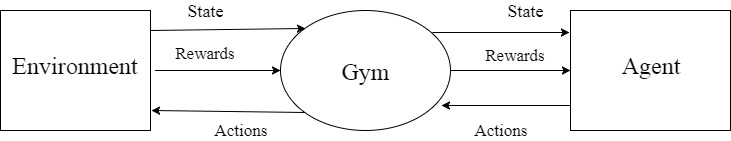
\includegraphics[width=\linewidth]{flow.jpg}
	\caption{Rough Flow of the algorithm}

\end{figure}
We will first try to implement a simple neural network for learning the
Q-functionfor a single player and increase it to two or more players. We will use its performance metrics as a baseline to compare further algorithms.  \newline\par


\subsection{Additional Objective}
\begin{itemize}
	\item{Explore rotational invariance: The training algorithm will see only a
  small square section of the environment. Since the viewpoint is square, the
  strategy should be invariant to 90 (degree) rotation. Therefore it can be
  considered that the snake is always moving above. This can potentially
  reduce the search space by a factor of 4 and reduce learning time.}
	\item{Prevent self-play instability: It may happen that the snakes, in
  order to survive, choose a particular region of the board and stay local
  to it (eat food and avoid boundary). The game may continue indefinitely
  without a decisive result. }
\end{itemize}
\section*{}

\begin{thebibliography}{00}
\bibitem{sp1} Watkins, C.J. and Dayan, P., 1992. Q-learning. Machine learning, 8(3-4), pp.279-292.
\bibitem{sp2} Tan, M., 1993. Multi-agent reinforcement learning: Independent vs. cooperative agents. In Proceedings of the tenth international conference on machine learning (pp. 330-337).
\bibitem{sp3} Mnih, V., Kavukcuoglu, K., Silver, D., Graves, A., Antonoglou, I., Wierstra, D. and Riedmiller, M., 2013. Playing atari with deep reinforcement learning. arXiv preprint arXiv:1312.5602.
\bibitem{sp4} Van Hasselt, H., Guez, A. and Silver, D., 2016, February. Deep Reinforcement Learning with Double Q-Learning. In AAAI (Vol. 16, pp. 2094-2100).
\bibitem{sp5} Schaul, T., Quan, J., Antonoglou, I. and Silver, D., 2015. Prioritized experience replay. arXiv preprint arXiv:1511.05952.
\bibitem{sp6} Wang, Z., Schaul, T., Hessel, M., Van Hasselt, H., Lanctot, M. and De Freitas, N., 2015. Dueling network architectures for deep reinforcement learning. arXiv preprint arXiv:1511.06581.
\bibitem{sp7} Silver, D., Huang, A., Maddison, C.J., Guez, A., Sifre, L., Van Den Driessche, G., Schrittwieser, J., Antonoglou, I., Panneershelvam, V., Lanctot, M. and Dieleman, S., 2016. Mastering the game of Go with deep neural networks and tree search. nature, 529(7587), pp.484-489.
\bibitem{sp8} Silver, D., Schrittwieser, J., Simonyan, K., Antonoglou, I., Huang, A., Guez, A., Hubert, T., Baker, L., Lai, M., Bolton, A. and Chen, Y., 2017. Mastering the game of go without human knowledge. Nature, 550(7676), p.354.
\bibitem{sp9} Bansal, T., Pachocki, J., Sidor, S., Sutskever, I. and Mordatch, I., 2017. Emergent complexity via multi-agent competition. arXiv preprint arXiv:1710.03748.
\bibitem{sp10} OpenAI. (August 2017). Dota 2. [online] Available at: https://blog.openai.com/dota-2/ [Accessed 1 Feb. 2018].
\bibitem{sd1} G. Brockman, V. Cheung, L. Pettersson, J. Schneider, J. Schulman, J. Tang, and W. Zaremba. OpenAI
Gym. arXiv preprint arXiv:1606.01540, 2016.
\bibitem{sd2} http://slither.io/
\bibitem{sd3} Mnih, V., Kavukcuoglu, K., Silver, D., Graves, A., Antonoglou, I., Wierstra, D., et al. (2013). ``Playing Atari with deep reinforcement learning." Technical report. Deepmind Technologies, arXiv:1312.5602 [cs.LG]
\bibitem{sd4} Bansal, T., Pachocki, J., Sidor, S., Sutskever, I., Mordatch, I.: ``Emergent complexity
via multi-agent competition." CoRR abs/1710.03748 (2017)
\bibitem{sd5} Qicheng Ma, Hadon Nash, ``Solving Multiplayer Games with Reinforcement Learning,"
\bibitem{sd6} Silver, A. Huang, C. J. Maddison, A. Guez, L. Sifre, G. Van Den Driessche, J. Schrittwieser, I. Antonoglou, V. Panneershelvam, M. Lanctot, et al. ``Mastering the game of go with deep neural networks and tree search," Nature, 529(7587):484–489, 2016.
\bibitem{n1}{1606.01540,Greg Brockman, Vicki Cheung, Ludwig Pettersson, Jonas Schneider, John Schulman, Jie Tang and Wojciech Zaremba,OpenAI Gym,2016}
\bibitem{n2}https://www.tensorflow.org
\bibitem{n3} {https://blog.openai.com/requests-for-research-2/}
\end{thebibliography}

\end{document}
